%%%%%%%%%%%%%%%%%%%%%%%%%%%%%%%%%%%%%%%%%%%%%%%%%%%%%%%%%%%%%%%%
%
%  Template for homework of Introduction to Machine Learning.
%
%  Fill in your name, lecture number, lecture date and body
%  of homework as indicated below.
%
%%%%%%%%%%%%%%%%%%%%%%%%%%%%%%%%%%%%%%%%%%%%%%%%%%%%%%%%%%%%%%%%


\documentclass[11pt,letter,notitlepage]{article}
%Mise en page
\usepackage[left=2cm, right=2cm, lines=45, top=0.8in, bottom=0.7in]{geometry}
\usepackage{fancyhdr}
\usepackage{fancybox}
\usepackage{graphicx}
\usepackage{pdfpages} 
\usepackage{enumitem}
\usepackage{algorithm}
\usepackage{algorithmic}
\renewcommand{\headrulewidth}{1.5pt}
\renewcommand{\footrulewidth}{1.5pt}
\newcommand\Loadedframemethod{TikZ}
\usepackage[framemethod=\Loadedframemethod]{mdframed}

\usepackage{amssymb,amsmath}
\usepackage{amsthm}
\usepackage{thmtools}
\newtheorem{lemma}{Lemma}

\setlength{\topmargin}{0pt}
\setlength{\textheight}{9in}
\setlength{\headheight}{0pt}

\setlength{\oddsidemargin}{0.25in}
\setlength{\textwidth}{6in}

\usepackage{graphicx} % more modern
\usepackage{subfigure}
\usepackage{ctex}

%%%%%%%%%%%%%%%%%%%%%%%%
%%%%%% Define math operator %%%%%
%%%%%%%%%%%%%%%%%%%%%%%%
\DeclareMathOperator*{\argmin}{\bf argmin}
\DeclareMathOperator*{\relint}{\bf relint\,}
\DeclareMathOperator*{\dom}{\bf dom\,}
\DeclareMathOperator*{\intp}{\bf int\,}
%%%%%%%%%%%%%%%%%%%%%%%


\setlength{\topmargin}{0pt}
\setlength{\textheight}{9in}
\setlength{\headheight}{0pt}

\setlength{\oddsidemargin}{0.25in}
\setlength{\textwidth}{6in}
\pagestyle{fancy}
%%%%%%%%%%%%%%%%%%%%%%%%
%% Define the Exercise environment %%
%%%%%%%%%%%%%%%%%%%%%%%%
\mdtheorem[
topline=false,
rightline=false,
leftline=false,
bottomline=false,
leftmargin=-10,
rightmargin=-10
]{exercise}{\textbf{Exercise}}
%%%%%%%%%%%%%%%%%%%%%%%
%% End of the Exercise environment %%
%%%%%%%%%%%%%%%%%%%%%%%


%%%%%%%%%%%%%%%%%%%%%%%%
%% Define the Problem environment %%
%%%%%%%%%%%%%%%%%%%%%%%%
\mdtheorem[
topline=false,
rightline=false,
leftline=false,
bottomline=false,
leftmargin=-10,
rightmargin=-10
]{problem}{\textbf{Problem}}
%%%%%%%%%%%%%%%%%%%%%%%
%% End of the Exercise environment %%
%%%%%%%%%%%%%%%%%%%%%%%

%%%%%%%%%%%%%%%%%%%%%%%
%% Define the Solution Environment %%
%%%%%%%%%%%%%%%%%%%%%%%
\declaretheoremstyle
[
spaceabove=0pt, 
spacebelow=0pt, 
headfont=\normalfont\bfseries,
notefont=\mdseries, 
notebraces={(}{)}, 
headpunct={:\quad}, 
headindent={},
postheadspace={ }, 
postheadspace=4pt, 
bodyfont=\normalfont, 
qed=$\blacksquare$,
preheadhook={\begin{mdframed}[style=myframedstyle]},
	postfoothook=\end{mdframed},
]{mystyle}

\declaretheorem[style=mystyle,title=Solution,numbered=no]{solution}
\mdfdefinestyle{myframedstyle}{%
	topline=false,
	rightline=false,
	leftline=false,
	bottomline=false,
	skipabove=-6ex,
	leftmargin=-10,
	rightmargin=-10}
%%%%%%%%%%%%%%%%%%%%%%%
%% End of the Solution environment %%
%%%%%%%%%%%%%%%%%%%%%%%

%% Homework info.
\newcommand{\posted}{\text{Nov. 5, 2019}}       			%%% FILL IN POST DATE HERE
\newcommand{\due}{\text{Nov. 18, 2019}} 			%%% FILL IN Due DATE HERE
\newcommand{\hwno}{\text{4}} 		           			%%% FILL IN LECTURE NUMBER HERE


%%%%%%%%%%%%%%%%%%%%
%% Put your information here %%
%%%%%%%%%%%%%%%%%%%
\newcommand{\name}{\text{Jiahuan Yu}}  	          			%%% FILL IN YOUR NAME HERE
\newcommand{\id}{\text{PB17121687}}		       			%%% FILL IN YOUR ID HERE
%%%%%%%%%%%%%%%%%%%%
%% End of the student's info %%
%%%%%%%%%%%%%%%%%%%


\newcommand{\proj}[2]{\textbf{P}_{#2} (#1)}
\newcommand{\lspan}[1]{\textbf{span}  (#1)  }
\newcommand{\rank}[1]{ \textbf{rank}  (#1)  }
\newcommand{\RNum}[1]{\uppercase\expandafter{\romannumeral #1\relax}}


\lhead{
	\textbf{\name}
}
\rhead{
	\textbf{\id}
}
\chead{\textbf{
		Homework \hwno
}}


\begin{document}
\vspace*{-4\baselineskip}
\thispagestyle{empty}


\begin{center}
	{\bf\large Introduction to Machine Learning}\\
	{Fall 2019}\\
	University of Science and Technology of China
\end{center}

\noindent
Lecturer: Jie Wang  			 %%% FILL IN LECTURER HERE
\hfill
Homework \hwno
\\
Posted: \posted
\hfill
Due: \due
\\
Name: \name
\hfill
ID: \id
\hfill

\noindent
\rule{\textwidth}{2pt}

\medskip





%%%%%%%%%%%%%%%%%%%%%%%%%%%%%%%%%%%%%%%%%%%%%%%%%%%%%%%%%%%%%%%%
%% BODY OF HOMEWORK GOES HERE
%%%%%%%%%%%%%%%%%%%%%%%%%%%%%%%%%%%%%%%%%%%%%%%%%%%%%%%%%%%%%%%%

\textbf{Notice, }to get the full credits, please show your solutions step by step.

\begin{exercise}[Support Vector Machine (SVM) for Linearly Separable Cases \textnormal{40pts}]
	Given the training sample $\mathcal{D}=\{ (\textbf{x}_i,y_i) \}_{i=1}^n$, where $\textbf{x}_i \in \mathbb{R}^d$ and $y_i \in \{ -1,1 \}$. Let
	\begin{align*}
		\mathcal{D}^+=\{(\textbf{x}_i,y_i)\in\mathcal{D}:y_i=1\},\hspace{5mm}\mathcal{D}^-=\{(\textbf{x}_i,y_i)\in\mathcal{D}:y_i=-1\}.
	\end{align*}
	Assume that $\mathcal{D}^+$ and $\mathcal{D}^-$ are nonempty and the training sample $\mathcal{D}$ is linearly separable. We have shown in class that SVM can be written as
	\begin{align}\label{prob:SVM-1}
		 & \min_{\textbf{w},b}\,\,\frac{1}{2}\| \textbf{w} \|^2,                                      \\
		 & \text{ s.t. } \min_i y_{i} ( \langle \textbf{w}, \textbf{x}_i \rangle + b ) = 1. \nonumber
	\end{align}
	Moreover, we further transform the problem in (\ref{prob:SVM-1}) to
	\begin{align}\label{prob:SVM}
		 & \min_{\textbf{w},b}\,\,\frac{1}{2}\| \textbf{w} \|^2,                                                    \\
		 & \text{ s.t. }\,\, y_{i} ( \langle \textbf{w}, \textbf{x}_i \rangle + b ) \geq 1, i=1,\ldots,n. \nonumber
	\end{align}
	We denote the feasible set of the problem in (\ref{prob:SVM}) by $$\mathcal{F}=\{(\mathbf{w},b):y_{i} ( \langle \textbf{w}, \textbf{x}_i \rangle + b ) \geq 1, i=1,\ldots,n\}.$$

	\begin{enumerate}
		\item Show that $\mathcal{F}$ is nonempty.
		\item Show that the problem in (\ref{prob:SVM}) admits an optimal solution.
		\item Let $(\textbf{w}^*,b^*)$ be the optimal solution to problem (\ref{prob:SVM}). Show that $\mathbf{w}^*\neq0$.
		\item Show that the problems in (\ref{prob:SVM-1}) and (\ref{prob:SVM}) are equivalent, that is, they share the same set of optimal solutions.
		\item Let $(\textbf{w}^*,b^*)$ be the optimal solution to problem (\ref{prob:SVM}). Show there exist at least one positive sample and one negative sample, respectively, such that the equality holds. In other words, there exist $i,j \in \{ 1,2,\dots,n \}$ such that
		      \begin{align*}
			      1=y_i =  & \langle \textbf{w}^*, \textbf{x}_i \rangle + b^*, \\
			      -1=y_j = & \langle \textbf{w}^*, \textbf{x}_j \rangle + b^*.
		      \end{align*}
		\item Show that the optimal solution to problem (\ref{prob:SVM}) is unique.
		\item Find the dual problem of (\ref{prob:SVM}) and the corresponding optimal conditions.
	\end{enumerate}

\end{exercise}
\begin{solution}

\end{solution}

\newpage
\begin{exercise}[Visualization Lemma]
	Consider the primal problem as follows.
	\begin{align}\label{prob:primal-vec}
		\min_{\mathbf{x}}\, & f(\mathbf{x})                \\ \nonumber
		{\rm s.t.}\,        & \mathbf{g}(\mathbf{x})\leq0, \\ \nonumber
		                    & \mathbf{h}(\mathbf{x})=0,    \\ \nonumber
		                    & \mathbf{x}\in X,
	\end{align}
	where $\mathbf{x}\in\mathbb{R}^n$, $f:\mathbb{R}^n\rightarrow\mathbb{R}$, $\mathbf{g}:\mathbb{R}^n\rightarrow\mathbb{R}^m$, $\mathbf{h}:\mathbb{R}^n\rightarrow\mathbb{R}^p$, and $X\subseteq\mathbb{R}^n$. The functions $f$, $\mathbf{g}$, and $\mathbf{h}$ are continuously differentiable.

	The Lagrangian $L:\mathbb{R}^n\times \mathbb{R}^m\times \mathbb{R}^p\rightarrow\mathbb{R}$ associated with the problem in (\ref{prob:primal-vec}) takes the form of
	\begin{align}\label{def:Lagrangian}
		L(\mathbf{x},\lambda,\mu)=f(\mathbf{x})+\sum_{i=1}^m\lambda_ig_i(\mathbf{x})+\sum_{i=1}^p\mu_ih_i(\mathbf{x}).
	\end{align}

	Let
	\begin{align}\label{def:image-set}
		\mathbb{R}^{m+p+1}\supseteq S=\{(\mathbf{g}(\mathbf{x}),\mathbf{h}(\mathbf{x}),f(\mathbf{x})):\mathbf{x}\in X\}.
	\end{align}

	Show that the results as follows (hint: see Fig. \ref{fig:visualization-lemma}).

	\begin{lemma}
		\textbf{\textup {Visualization Lemma}}
		\begin{enumerate}
			\item The hyperplane with normal $(\lambda,\mu,1)$ that passes through a vector $(\mathbf{g}(\mathbf{x}),\mathbf{h}(\mathbf{x}),f(\mathbf{x}))$ intercepts the vertical axis $\{(\mathbf{0},z):z\in\mathbb{R}\}$ at the level $L(\mathbf{x},\lambda,\mu)$.

			\item Among all hyperplanes with normal $(\lambda,\mu,1)$ that contains in their positive halfspace the set $S$ defined in (\ref{def:image-set}), the highest attained level of interception of the vertical axis is $\inf_{\mathbf{x}\in X}\,L(\mathbf{x},\lambda,\mu)$.

			\item $(\lambda^*,\mu^*)$ is a geometric multiplier if and only if $\lambda^*\geq0$ and among all hyperplanes with normal $(\lambda^*,\mu^*,1)$ that contain in their positive halfspace the set $S$, the highest attained level of of interception of the vertical axis is $f^*$, where
			      \begin{align*}
				      f^*=\min\{f(\mathbf{x}):\mathbf{g}(\mathbf{x})\leq0,\mathbf{h}(\mathbf{x})=0,\mathbf{x}\in X)\}.
			      \end{align*}
		\end{enumerate}
	\end{lemma}
\end{exercise}
\begin{figure}[!h]
	\centering{
		\subfigure[] { \label{fig:geometric-multiplier-0}
			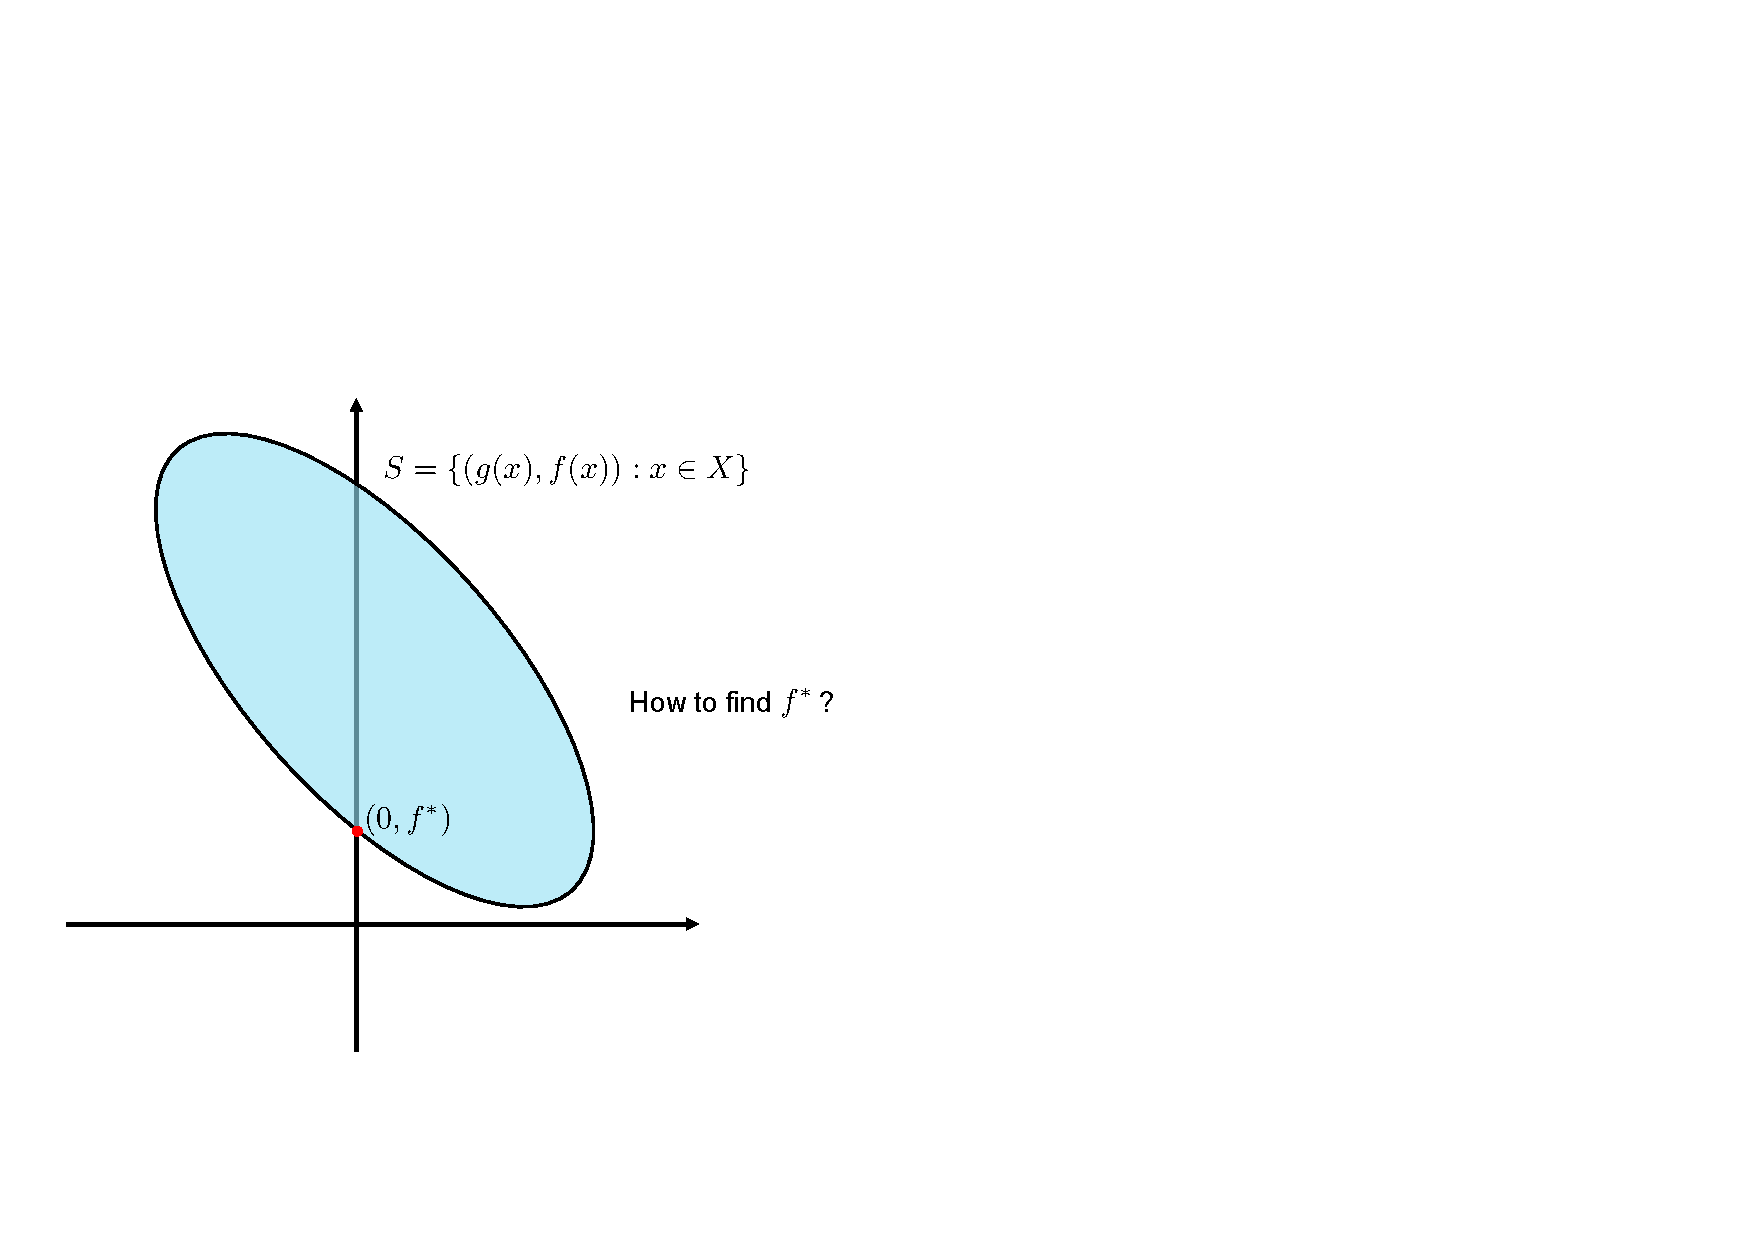
\includegraphics[width=0.45\columnwidth]{figures/geometric-multipliers-0.pdf}
		}
		\subfigure[] { \label{fig:geometric-multiplier-1}
			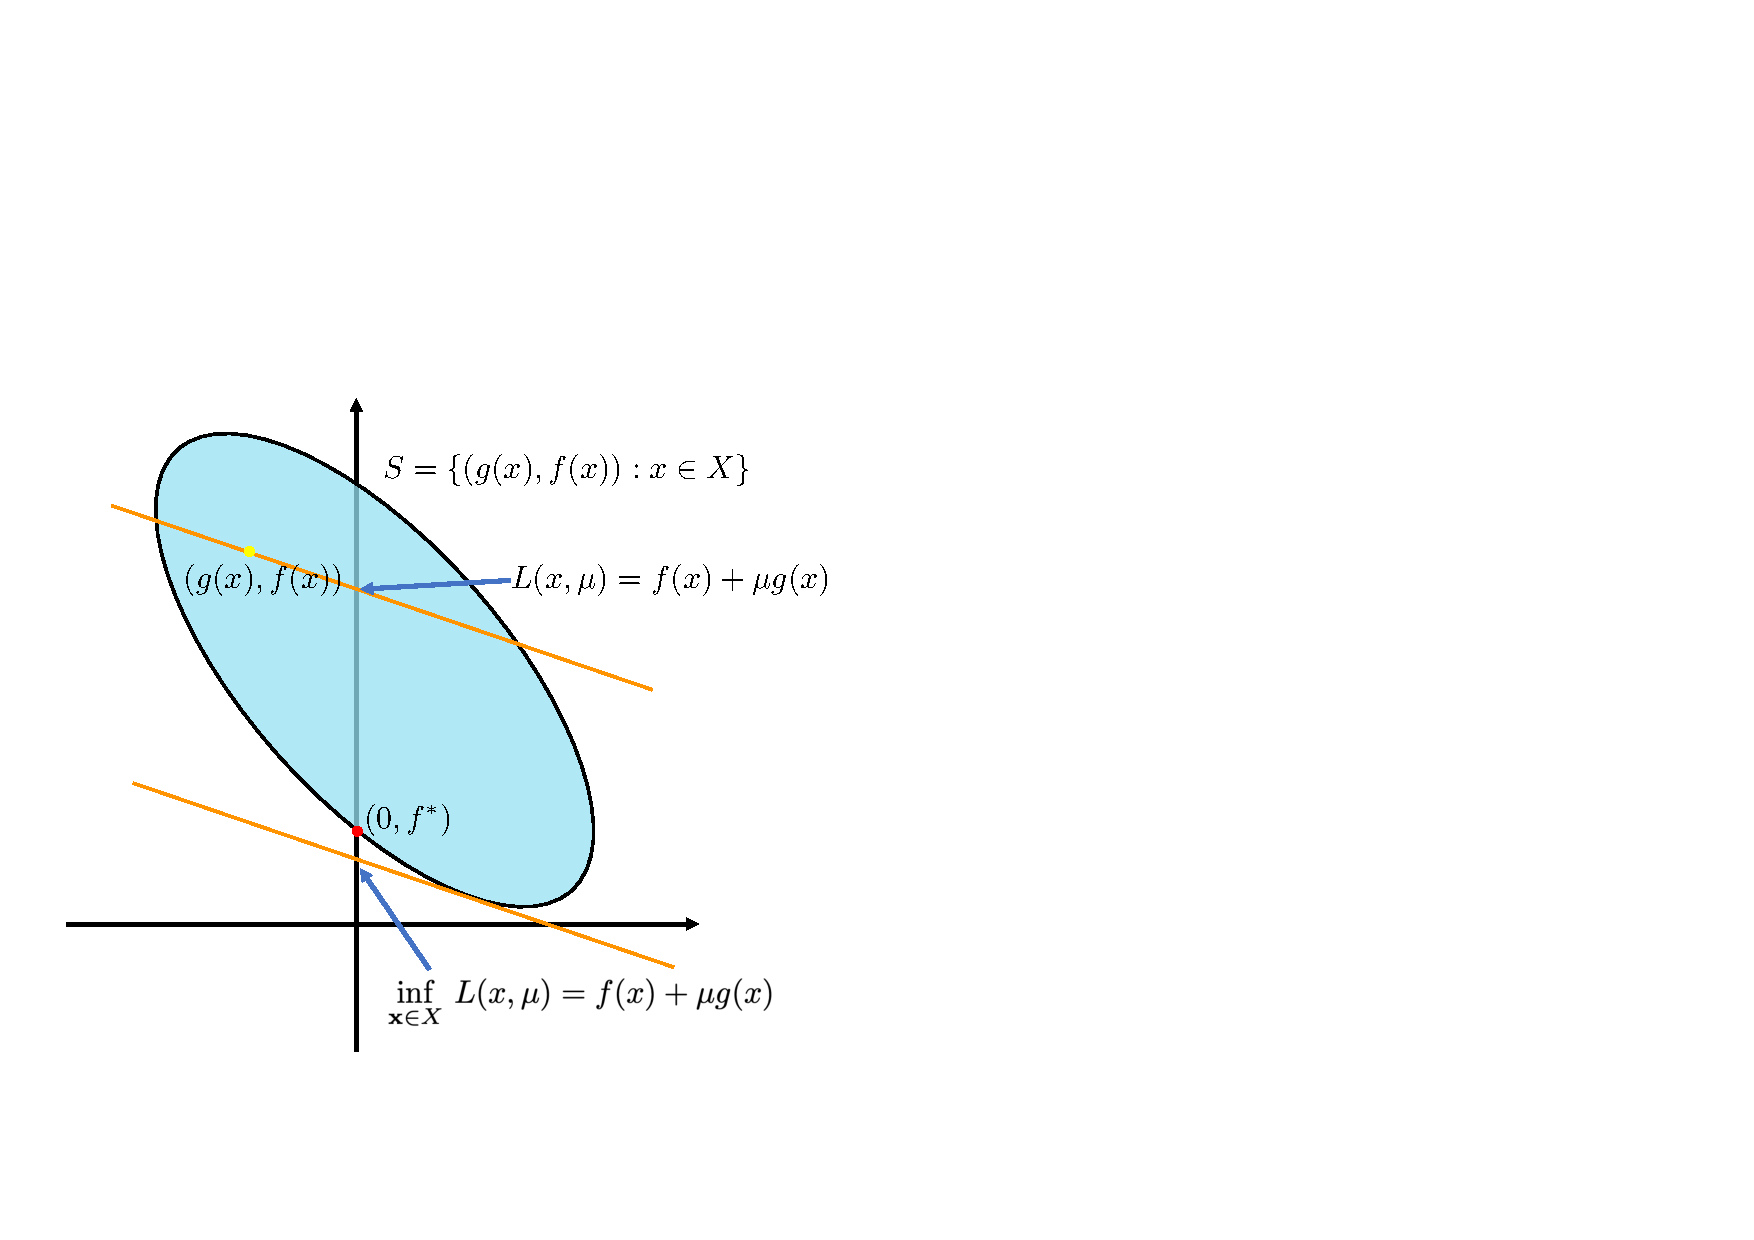
\includegraphics[width=0.45\columnwidth]{figures/geometric-multipliers-1.pdf}
		}
	}
	\caption{Illustration of the visualization lemma with one inequality constraint.}
	\label{fig:visualization-lemma}
\end{figure}



\newpage
${}$
\newpage
\begin{exercise}[Geometric Multiplier]
	Let $(\lambda^*,\mu^*)$ be a geometric multiplier. Show that $\mathbf{x}^*$ is a global minimum of the primal problem (\ref{prob:primal-vec}) if and only if $\mathbf{x}^*$ is feasible and
	\begin{align*}
		 & \mathbf{x}^*\in\argmin_{\mathbf{x}\in X}\,L(\mathbf{x},\lambda^*,\mu^*), \\
		 & \lambda_i^*g_i(\mathbf{x}^*)=0,\,i=1,\ldots,m.
	\end{align*}
\end{exercise}

\newpage
\begin{exercise}[Lagrange Dual Problem]
	Consider the primal problem (\ref{prob:primal-vec}) and the Lagrangian (\ref{def:Lagrangian}). We define the dual function for $(\lambda,\mu)\in\mathbb{R}^{m+p}$ by
	\begin{align*}
		q(\lambda,\mu)=\inf_{\mathbf{x}\in X}\,L(\mathbf{x},\lambda,\mu).
	\end{align*}
	The domain of $q$ is
	\begin{align*}
		\dom(q)=\{(\lambda,\mu):q(\lambda,\mu)>-\infty\}.
	\end{align*}
	The dual problem is
	\begin{align*}
		\sup\,       & q(\lambda,\mu), \\
		\mbox{s.t. } & \lambda\geq0.
	\end{align*}
	\begin{enumerate}
		\item Show that $\dom(q)$ is convex.
		\item Show that $-q(\lambda,\mu)$ is a convex function.
	\end{enumerate}
\end{exercise}





\newpage
\begin{exercise}[Duality Gap]
	Duality gap is defined by
	\begin{align*}
		f^*-q^*.
	\end{align*}
	Show that the following results hold.
	\begin{enumerate}
		\item If there is no duality gap, the set of geometric multipliers is equal to the set of optimal dual solutions.
		\item If there is duality gap, the set of geometric multipliers is empty.
	\end{enumerate}
\end{exercise}

\newpage
\begin{exercise}[Optimality Conditions]
	Show that a pair $\mathbf{x}^*$ and $(\lambda^*,\mu^*)$ is an optimal solution and geometric multiplier pair if and only if
	\begin{align}\label{cond:primal-feasibility}
		\mathbf{x}^*\in X,\,\mathbf{g}(\mathbf{x}^*)\leq0,\mathbf{h}(\mathbf{x}^*)=0,\hspace{18.5mm}(\mbox{\textup{Primal Feasibility}}), & \\ \label{cond:dual-feasibility}
		\lambda^*\geq0,\hspace{22mm}(\mbox{\textup{Dual Feasibility}}),                                                                   & \\ \label{cond:lagrangian-optimality}
		\mathbf{x}^*\in\argmin_{\mathbf{x}\in X}\,L(\mathbf{x},\lambda^*,\mu^*),\hspace{10mm}(\mbox{\textup{Lagrangian Optimality}}),     & \\ \label{cond:complementary-slackness}
		\lambda^*_ig_i(\mathbf{x}^*)=0,\,i=1,\ldots,m,\hspace{5mm}(\mbox{\textup{Complementary Slackness}}).                              &
	\end{align}
\end{exercise}


\newpage
\begin{exercise}[Saddle Point Interpretation]
	Show that a pair $\mathbf{x}^*$ and $(\lambda^*,\mu^*)$ is an optimal solution-geometric multiplier pair if and only if $\mathbf{x}^*\in X$, $\lambda^*\geq0$, and $(\mathbf{x}^*,\lambda^*,\mu^*)$ is a saddle point of the Lagrangian, in the sense that
	\begin{align}\label{cond:saddle-Lagrangian}
		L(\mathbf{x}^*,\lambda,\mu)\leq L(\mathbf{x}^*,\lambda^*,\mu^*)\leq L(\mathbf{x},\lambda^*,\mu^*),\,\forall\,\mathbf{x}\in X,\,\lambda\geq0.
	\end{align}
\end{exercise}


\newpage
\begin{exercise}
	Recall that the soft margin SVM takes the form of
	\begin{align}\label{prob:soft-SVM}
		\min_{\mathbf{w},b,\xi}\, & \frac{1}{2}\|\mathbf{w}\|^2+C\sum_{i=1}^n\xi_i,                           \\ \nonumber
		{\rm s.t.\,}              & \,y_i(\langle\mathbf{w},\mathbf{x}_i\rangle+b)\geq1-\xi_i,i=1,\ldots,n, & \\ \nonumber
		                          & \,\xi_i\geq0,\,i=1,\ldots,n,
	\end{align}
	where $C>0$.
	The corresponding dual problem is
	\begin{align}\label{prob:dual-soft-SVM}
		\min_{\alpha}\, & \frac{1}{2}\sum_{i=1}^n\sum_{j=1}^n\,\alpha_i\alpha_jy_iy_j\langle\mathbf{x}_i,\mathbf{x}_j\rangle-\sum_{i=1}^n\alpha_i \\\nonumber
		\mbox{s.t. }\,  & \sum_{i=1}^n\alpha_iy_i=0,                                                                                              \\\nonumber
		                & \alpha_i\in[0,C],i=1,\ldots,n.
	\end{align}
	\begin{enumerate}
		\item Show that the problems (\ref{prob:soft-SVM}) and (\ref{prob:dual-soft-SVM}) always admit optimal solutions.

		\item Suppose that the training data consists of two data instances $x_1=1$ and $x_2=-1$, and the corresponding labels are $y_1=1$ and $y_2=-1$.
		      \begin{enumerate}
			      \item Please solve problem (\ref{prob:SVM}) and find the primal and dual optimal solutions.
			      \item Please solve problem (\ref{prob:soft-SVM}) with $C<\frac{1}{2}$ and find the primal and dual optimal solutions.
		      \end{enumerate}

		\item Suppose that the training data consists of four data instances: $\mathbf{x}_1=(2,3)$, $\mathbf{x}_2=(1,2)$, $\mathbf{x}_3=(1,3)$, and $\mathbf{x}_4=(2,2)$, and the corresponding labels are $y_1=y_2=1$ and $y_3=y_4=-1$. Please solve the problem in (\ref{prob:dual-soft-SVM}) with $C=10$.
	\end{enumerate}
	Notice that, for the last two parts, you need to find all the primal and dual optimal solutions if they are not unique.
\end{exercise}

%%%%%%%%%%%%%%%%%%%%%%%%%%%%%%%%%%%%%%%%%%%%%%%%%%%%%%%%%%%%%%%%

\end{document}
